% This is LLNCS.DEM the demonstration file of
% the LaTeX macro package from Springer-Verlag
% for Lecture Notes in Computer Science,
% version 2.4 for LaTeX2e as of 16. April 2010
%
\documentclass[oribibl]{llncs}
%
\usepackage{makeidx}  % allows for indexgeneration

%%%%%CUSTOM PACKAGES%%%%%
\usepackage{graphicx}
\usepackage{float}
\usepackage{color}
\usepackage[usenames,dvipsnames]{xcolor}
\usepackage{framed}
\usepackage[utf8]{inputenc}

\usepackage{alltt}
\renewcommand{\ttdefault}{txtt}

%%%FOR LATEXDRAW %%%%
 \usepackage[usenames,dvipsnames]{pstricks}
 \usepackage{epsfig}
 \usepackage{pst-grad} % For gradients
 \usepackage{pst-plot} % For axes



%%%%%%
%
\begin{document}
%
\frontmatter          % for the preliminaries
%
\pagestyle{headings}  % switches on printing of running heads
\addtocmark{Controlled languages for artificial cognition} % additional mark in the TOC
\title{Controlled Natural Languages in\\ Artificial Cognition: Uncertainty Verbalization\\and Language Generation}
%
\titlerunning{Controlled languages in artificial cognition}  % abbreviated title (for running head)
%                                     also used for the TOC unless
%                                     \toctitle is used
\author{Nicholas H. Kirk$^1$, Daniel Nyga$^{1,2}$, Michael Beetz$^2$}
%
\authorrunning{Kirk et al.} % abbreviated author list (for running head)
%
%%%% list of authors for the TOC (use if author list has to be modified)
\tocauthor{Nicholas H. Kirk$^1$, Daniel Nyga$^1$, Michael Beetz$^2$}
%
\institute{$^1$Intelligent Autonomous Systems, Technische Universität München, Germany\\
$^2$Institute for Artificial Intelligence \& TZI\footnote{The Center for Computing Technologies (TZI)}, University of Bremen, Germany
\email{nicholas.kirk@tum.de}, \email{nyga@cs.tum.edu}, \email{beetz@cs.uni-bremen.de}
}
\maketitle              % typeset the title of the contribution
\begin{abstract}

%In this paper we discuss the problem of action-specific knowledge processing, representation and acquisition
%by autonomous robots performing everyday activities.
In this paper we discuss, within the context of artificial assistants performing everyday activities, a resolution method to disambiguate missing or not satisfactorily inferred action-specific information via explicit clarification.
%Within the context of artificial assistants in Information related to the latter is often incomplete, requires 
%disambiguation and inference. However, this can still be insufficient and require explicit clarification. 
While arguing the lack of preexisting human-robot interaction means, 
we introduce novel uses of Controlled Natural Languages (CNL)
as means of linguistic human-robot interaction and action-oriented representation formalization.\\
We additionally provide implemented working scenarios, 
state future possibilities and problems related to formalization of technical cognition.

\keywords{language generation, action formalization, controlled 
natural language, intelligent autonomous systems, probabilistic 
robot action cores, discourse representation structures, attempto 
controlled english} \end{abstract}

\section{Introduction} 

In everyday routine activities, robotic assistants and co-workers 
will have to perform a variety of tasks for which they cannot be 
pre-programmed because they are not known at production time. 
Research in the field of cognitive robotics rather envisions service 
robots that autonomously acquire new skills and adapt existing ones 
to new tasks and environments. They must decide on \textit{how} to 
perform a particular activity at runtime, which requires to infer 
the \textit{appropriate} actions to be executed on the \textit 
{appropriate} objects in an \textit{appropriate} way. They have to 
perform what is commonly referred to as \textit{everyday activity}, 
which has been proven to be a very knowledge-intensive task~\cite 
{anderson95phd, nyga12actioncore}. It requires context awareness and 
flexibility in action parameterization when operating in real world 
settings with partially available data, which is referred to as the 
``open world challenge.'' 

Recent research in the field of cognitive robotics aims at making 
knowledge sources available for robots, which have been created by 
humans and are intended for human use. For some domains such as 
daily household tasks (e.g. cooking or cleaning up), step-by-step 
plans and recipes from web pages like \textit {ehow.com} and \textit 
{wikihow.com} have been successfully used for feeding such common 
sense knowledge about actions and objects into knowledge bases of 
mobile robotic platforms and for transforming such recipes into 
executable robot plans~\cite{tenorth10webinstructions}. However, as 
these recipes are presented in natural language, severe ambiguity, 
vagueness and underspecification have been identified as major 
challenges in doing so. From a robotic assistant's standpoint, 
natural-language instructions from the web are very often severly 
incomplete and present knowledge understatement, since many missing 
key pieces of information are generally considered common sense to 
the human, and hence explicit statements of these kinds of 
self-evident yet necessary information are rendered obsolete. As an 
example, consider a natural-language instruction ``Flip the 
pancake,'' which might be taken from a recipe for making pancakes. 
In order to perform the action successfully, a robot needs to decide 
which utensil to use (e.g. a spatula), where to hold it (e.g. at its 
handle) and what part of it to put underneath the pancake (e.g. the 
blade), to name only a few.

Current research in cognitive robotics aims at building up action 
verb-specific knowledge bases that fill this gaps of knowledge and 
enable a robot to infer the information which is \textit{needed} in 
order to perform a particular activity, based on what is \textit 
{given} in a naturalistic action specification. However, such 
inference might incur in limitations and require the robot to fall 
back on human assistance. As an example, consider a situation where 
the robot is asked to flip a pancake, but the knowledge base does 
not contain sufficient information about what instrument to be used 
(e.g. it has no strong preference for a spatula over barbeque 
tongs). In such a case, the robot is to explicitly ask a human for 
further information. Figure \ref{fig:application} illustrates such a 
situation. Taxonomical and compositional relationships, object role 
understanding, are only some of the missing elements that could 
potentially require clarification. 


\begin{figure}[H]
%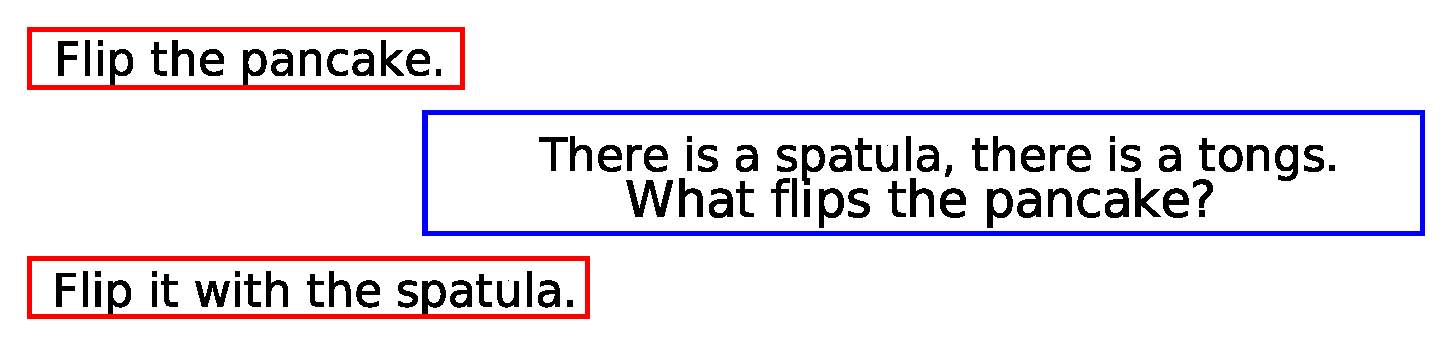
\includegraphics[width=.9\columnwidth]{introduction.eps}
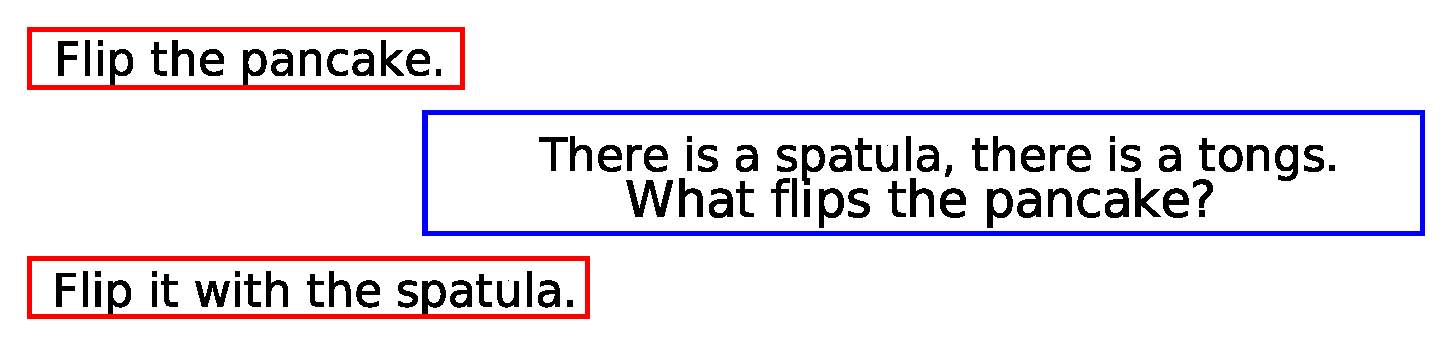
\includegraphics[scale=0.51, trim = 0mm 0mm 0mm 8mm]{introduction.eps}
\caption{Representation of a disambiguation interaction}
\label{fig:application}
\end{figure} 

In this work, we present a novel approach for identifying and 
verbalizing such lacks of information in a knowledge base in order to enable
a robot to acitively enhance its knowledge about actions and objects
by stepping into dialog with humans. 
\newpage
The contributions of this paper
are the following:
\begin{enumerate}
    \item use of CNL as means of language generation (i.e. verbalization of doubt statements and questions)
    \item use of CNL as means of action-oriented knowledge formalization
\end{enumerate}
The remainder of this paper is organized as follows: description of the adopted technologies (i.e. PRAC, ACE, DRS), 

\section{Probabilistic Robot Action Cores}

Nyga \emph{et al.}~\cite{nyga12actioncore} introduced the concept of 
\emph{Probabilistic Robot Action Cores} (PRAC), which can be thought as abstract,
generic event patterns representing sets of 
inter- and intraconceptual relations that constitute an abstract 
event type, assigning an action role to each entity that is affected 
by the respective action verb. Formally, a PRAC is defined as a conditional
probability distribution
$P\left(\mathcal{R}\times\mathcal{A}\times\mathcal{C}\,|\,\sqsubseteq
,\, \preceq \right)\nonumber$, where 

\begin{center} \begin{tabular}{ll}
    $\mathcal{R}$  & is the set of all action roles\\
    $\mathcal{A}$  & is the set of all action verbs\\
    $\mathcal{C}$  & is the set of all class concepts\\
    %$P$ &  \text{is a probability distribution}\\
	%&  \text{over all role assignments of an action}\\
    %$\pi$ &  $\pi:\mathcal{A}\rightarrow 2^{\mathcal{R}}$ \text{ is a function that selects}\\
    %& \text{the needed roles given an action}\\
    $\sqsubseteq$ & is a taxonomy relation over $\mathcal{C}$\\
    $\preceq$	& is a mereological relation over $\mathcal{C}$.
\end{tabular}
\end{center}
As opposed to most approaches towards understanding natural-language 
instructions, which merely seek to understand what is given by an 
instruction, the PRAC concept is also able to infer what is missing. 
It combines action-specific and ontological world knowledge in a 
joint probabilistic first-order representation, which allows to 
automatically find generalizations from concrete event occurrences 
at an appropriate level of abstraction. Specifically, PRAC models 
are represented as a set of action roles (objects involved in the 
action with a specific role) and Markov Logic Networks (MLN), a 
knowledge representation formalism that combines first-order logic 
and probability theory~\cite{DBLP:journals/ml/RichardsonD06}. In this
work, we use the definitions of Action Roles in order to identify and
verbalize insufficient information about action parameterization. For a 
detailed discussion of PRAC models, we refer to \cite{nyga12actioncore}.

\section{Attempto Controlled English \& Discourse Representation Structures}

Fuchs \textit{et al.}~\cite{fuchs:flairs2006} presented Attempto Controlled English (ACE), a general purpose Controlled Natural Language, i.e. a subset of standard English with a restricted syntax and restricted semantics described by a small set of construction and interpretation rules.
Being this a formal subset of the English language, it is intelligible as a natural language, can be paraphrased and proved by automatic theorem proving software, and furthermore can be translated into First Order Logic or OWL ontology representations.

ACE provides many language constructs such as countable nouns (e.g. 'man', 'water'), proper names ('John'); 
generalized quantifiers (‘at least 2’); indefinite pronouns (‘somebody’); intransitive, transitive and ditransitive verbs (‘sleep’, ‘like’, ‘give’); negation, conjunction and disjunction of noun phrases, verb phrases, relative clauses and sentences; and anaphoric references to noun phrases through definite noun phrases, pronouns, and variables.
An example: \begin{alltt}{\color{red} ACE:} "A robot who does not understand asks a human that knows."\end{alltt}

These sentences have a two-way relationship with Discourse Representation Structures (DRS), a format to encode information of multiple sentences, preserving anaphoric cross-references (i.e. \textit{discourse referents})~\cite{kamp1993discourse}.\\
A concrete example would be the following sentence-DRS couple: 
\begin{verbatim}
sentence: "A robot flips a pancake."
DRS: [x,y: robot(x), pancake(y), flips(x,y)]
\end{verbatim}

\section{Related work}
Recently ACE has been exploited for uses such as Semantic Web Ontologies~\cite{decoi2009rewerse}, Multilingual semantic wikis~\cite{kuhnkaljurandsemantic}, while this paper focuses on the contributions of ACE in the artificial cognition domain.
According to what is known to the authors to date, the verbalization functionality itself~\cite{kaljurand:phd} has been used uniquely for verbalizing existing Semantic Web content, specifically OWL ontologies.
While using the same means (i.e. the DRS verbalizer, an intermediate phase of the OWL verbalizer) we exploit the system for verbalizing questions and doubt statements, as an attempt to verbalize a probabilistic knowledge formalism, and as the formalization per se of action-oriented knowledge in the everyday context we described.

\section{CNL for task querying}
The PRAC system caters for inference of missing action roles. Unfortunately, this operation can be partially satisfactory and might require explicit verbal clarification, in order to avoid that partially inferred information is translated into action planning.
We identify the following interaction:
{\large
\begin{alltt}
\textbf{\color{Red}Human to Robot} : Tasking Instruction            (in NL)
\textbf{\color{Blue}Robot to Human} : Ambiguity Resolution Question (in CNL)
\textbf{\color{Red}Human to Robot} : Disambiguation Reply           (in NL)
\end{alltt}
}
The last two phases can be cycled until the robotic assistant reaches a sufficient level of understanding. 
Taxonomical, temporal, decision, impossibility clarifications are only some of the \textit{disambiguation cases} in which an explicit verbal task querying is necessary from the robot to the human. 
The generation of natural-like language is non-trivial mainly given the scalability issues of linguistic factors of the sentence construction (e.g. anaphora resolution, number/gender/particle concordance, subordinate sentence handling, punctuation, verb conjugation). These requirements have proven to be fulfilled by Attempto Controlled English, now used as means of sentence generation.\\
Specifically for an action-oriented representation, we present our cognitive verbalization procedure, operated for each non-assigned action role:

\begin{enumerate} %TODO I don't know how to put across the following in a clearer way
    \item identification of the \textit{disambiguation cases}  (i.e. type of doubt statement)\\
    \item articulation of such doubt statement encapsulating what was inferred, and an interrogative sentence (to query the object itself, knowing its syntactic type) \\ 
    \item integration of the reply, assigning the previously missing action roles 
\end{enumerate}

\paragraph{case identification} is performed via threshold evaluation of probability distributions of likely objects for the missing role. 
Possible reasons for which the role assignment is missing, is the impossibility of 
defining a likely candidate (all probability assignments are below a threshold) or identifying manifold candidates (probability assignments are too close), or
the optimal candidate is not available in context.  

\paragraph{sentence construction} is operated to provide a grammar structure and contextual information for the disambiguation case and is performed via pre-defined DRS template instantiation. 
\begin{alltt}
{\large \textsc{two-choices}}:
    \textbf{query_case}: doubt between two plausible objects
    \textbf{template}: There is a X1, there is a X2.
    \textbf{drs}: drs([A,B],[object(A,X1,countable,na,eq,1)-1/4,
    object(B,X2,countable,na,eq,1)-1/9])
    \textbf{dependencies}: PARAM1-ext, PARAM2-ext; X1, X2
\end{alltt}
The DRS templates are instantiated by substituting syntactically contextual information taken from the initial Natural Language Instruction, or from the inferred probability distribution of likely objects (i.e. dependencies).
This is then verbalized with the DRS$\Rightarrow$ACE verbalizer module, process that accounts for the linguistic issues described beforehand.\\
Having clarified the nature of the ambiguity (e.g. comparison, impossibility) the abstract case has to be followed by a question asking the object, given the syntactic type (e.g. asking for instrument, direct object, preposition from/to). The verbalization process for the latter follows the same procedure stated for the disambiguation cases. \\
This is done to provide the human with a better understanding of the uncertainty, namely the information that has been inferred (e.g. doubt between two objects) and the questioning of the object itself (e.g. "what instrument should be used?").  
The verbalization templates refer to one single syntactic instance: upon PRAC template model construction (an abstraction for all instances of that action verb, e.g. 'flipping') we define a \textit{controlled template}, an ACE sentence that comprises all uninstantiated action roles in a possible syntactic configuration.
For the example above:
{\small
\begin{alltt}
\textbf{controlled_template}: The INSTRUMENT flips the THEME from FIXEDLOCATION. 
\end{alltt}
}%TODO justify this line of text
This provides an understanding of all the relationships between the entities involved in the action (i.e. syntactic relationships).
This will be of use since all DRS templates will then refer to this possible syntactic formulation. The relationships from the latter are obtained by processing it with the Stanford Parser\cite{mcdm08b}, a typed syntactic parser.
Unknown syntactic types related to the missing roles are taken from the instantiated version of such sentence, that comprises the known roles so far, and queried.
The querying procedure is identical to the one above, via the use of similar templates.

%\begin{alltt}
%{\large \textsc{instrumental}}:

%        \textbf{query_case}: preposition of instrument
%        \textbf{template}: What X1 the X2?
%        \textbf{drs}: drs([],[question(drs([A,B,C],[query(A,what)-1/1,
%        object(C,X2,countable,na,eq,1)-1/4,
%        predicate(B,X1,A,C)-1/2]))])
%        \textbf{dependencies}: NSUBJ-left, NSUBJ-right; X1, X2
%\end{alltt}

%The system has proved scalability given also the aggregation capability of DRS.

\paragraph{reply integration} is handled by \textit{PRACInference}, a module that processes the incoming sentence and assigns action roles. We will then substitute only the newly identified action roles that were previously missing in the main PRAC instance.

By combining the disambiguation doubt and query verbalization we obtain:
\begin{alltt}
To be asked:
  - Ask for missing role \textbf{"Instrument"}, case \textbf{"two-choices"},
  - Ask for missing role \textbf{"Instrument"}, case \textbf{"nsubj"}  
\textbf{\color{red}
Verbalization: 
ACE: [[There is a spatula.],[There is a n:tongs.]]
ACE: [[What v:flips a pancake?]]
}
\end{alltt}
\section{CNL for action formalization}
For the formalization of a PRAC model, be it grounded or abstract, we require a format that can serialize the instance or generate the PRAC model template.
We therefore need a statement that comprises all generative information, namely all roles involved in the action and the data that can create the MLN templates.  

We create this by encapsulating the action roles as nouns in a Controlled Natural Language statement, for human-readability and for preserving the syntactic relationships between the objects; furthermore we add explicit semantic tags to maintain information regarding semantic disambiguation of objects.
An implementation is possible via the use of ACE and semantic tags from WordNet\cite{Miller95wordnet:a}. To pursue the example of above:
\begin{alltt}
\textbf{The AGENT.n.06 flips.v.08 the THEME.n.01 from LOCATION.n.01 \\with an INSTRUMENT.n.01.}
\end{alltt}
An example of the semantic information that is then retrievable:
{\small
\begin{alltt}
\textbf{agent.n.06} {\color{red}(the semantic role of the animate entity that instigates or 
causes the happening denoted by the verb in the clause)}
\end{alltt}}

\paragraph{template generation} will create, given the above generating sentence, an initial set of action roles and MLN formula templates.
An example of the target format for the action verb 'Flipping': 
  
{\scriptsize

\begin{verbatim}
  
action_core: Flipping
definition: An Agent causes a Theme to move with respect to a FixedLocation, 
generally with a certain Periodicity, without undergoing unbounded translational 
motion or significant alteration of configuration/shape.
inherits_from: CauseMotion
action_roles:
    - Theme:
        - definition: A physical entity that is participating in non-translational motion.
    - FixedLocation:
        - definition: The point or set of points that define the limits of motion for the
         Theme. For spinning motions, it is the axis, for vibrating it is a boundary, 
         for swinging it is a point. 
        - range: LocativeRelation
    - Instrument: An entity that is used to perform the flipping action.
action_verbs:
    - flip: flip.v.08
formula_templates:
    - "action_role(?w, +?role) ^ has_sense(?w, ?s) ^ is_a(?s, ?c)"
    - "has_pos(?w,+?pos) ^ action_role(?w, +?role)"
    - "has_sense(?w, ?s) ^ is_a(?s, NULL) => action_role(?w, NULL)"
    - "action_role(?w, +?r) ^ has_sense(?w, ?sid) ^ is_a(?sid, +?sense)"
    - "prep_with(?w1, ?w2) ^ action_role(?w1, +?role1) ^ action_role(?w2, +?role2)"
    - "prep_in(?w1, ?w2) ^ action_role(?w1, +?role1) ^ action_role(?w2, +?role2)"
    - "prep_on(?w1, ?w2) ^ action_role(?w1, +?role1) ^ action_role(?w2, +?role2)"
    - "dobj(?w1, ?w2) ^ action_role(?w1, +?role1) ^ action_role(?w2, +?role2)"
    - "dobj(?w1, ?w2) ^ prep_from(?w1, ?w3) ^ action_role(?w1, +?r1) ^ 
    action_role(?w2, +?r2) ^ action_role(?w3, +?r3)"
    - "dobj(?w1, ?w2) ^ prep_with(?w1, ?w3) ^ action_role(?w1, +?r1) ^ 
    action_role(?w2, +?r2) ^ action_role(?w3, +?r3)"
    - "dobj(?w1, ?w2) ^ prep_into(?w1, ?w3) ^ action_role(?w1, +?r1) ^ 
    action_role(?w2, +?r2) ^ action_role(?w3, +?r3)"
\end{verbatim}
}
The action roles correspond to the nouns of the generating sentence, and their type of syntactic relationship defines the variant MLN templates that evaluate the probability of all possible syntactic types the action roles can be involved in. Other lexicographical information such as descriptions can be retrieved via preexisting webservices.

\section{results, discussions and conclusions}
This paper brings attention to possible uses of Controlled Natural Languages in the artificial cognition domain. While already proven as powerful means of representation and reasoning for the semantic web\cite{kuhnkaljurandsemantic}, our claim is that novel uses are possible for robotic assistants, specifically as human-to-robot interface.
We have proved via practical implementations that CNL can be exploited as means of language generation and presented current work in progress in relation to full action-oriented cognitive formalization.

However, even if it is a facilitated mean of knowledge engineering, CNL construction is not always straightforward\cite{Schwitter05alayered}. Infact, the DRS construction of the disambiguation cases had to account for the ACE construction rules (that can present expressiveness limitations) and the asymmetry of what is accepted as correct ACE statement and what can be verbalized (e.g. modals). Being the system purely a DRS\cite{drslatest} and PRAC based syntactical manipulator, the verbalizer is constrained by the current implemented features of these and presents similar limitations. This is visible since the system outputs are readable but not perfectly natural-like sentences, and on the other hand we have scalability issues given by improper object probability inference.
%The practical implementation of a PRAC model template generator will provide insights regarding representation limitations, for now discussed only theoretically. 
With the expansion of the expressiveness set of ACE and DRS, future work will aim towards how to make use of such abstractions in order to provide robotic assistants with further means of expression.
Further research will also be dedicated to the interaction dialogue itself and to \textit{learning via human-robot verbal interaction}, made possible via template generation and further knowledge manipulation, thanks to the common ground of Controlled Natural Languages.

% ---- Bibliography ----
%
\bibliography{bibform}{}
\bibliographystyle{unsrt}
%\clearpage
%\addtocmark[2]{Author Index} % additional numbered TOC entry
%\renewcommand{\indexname}{Author Index}
%\printindex
%\clearpage
%\addtocmark[2]{Subject Index} % additional numbered TOC entry
%\markboth{Subject Index}{Subject Index}
%\renewcommand{\indexname}{Subject Index}
%\input{subjidx.ind}
\end{document}
